\documentclass{article}
\usepackage[T1]{fontenc}
\usepackage{lmodern}
\usepackage{graphicx}
\usepackage{amsmath,amssymb}
\usepackage[a4paper,margin=2cm]{geometry}
\usepackage[absolute,overlay]{textpos}
\setlength{\TPHorizModule}{1mm}
\setlength{\TPVertModule}{1mm}
\usepackage[indonesian]{babel}
\usepackage{hyperref}
\setlength{\emergencystretch}{2em}
% unit: Halaman 16

\begin{document}

% === Halaman 16 (llm) ===

\vspace{196.02mm}

\begin{center}
\huge Pembangkitan kunci internal secara lengkap:
\end{center}

\vspace{80mm}

\begin{flushright}
Sumber: Cryptography\
and Network Security\
Chapter 3, Lecture slides\
by Lawrie Brown\
Modified by Richard\
Newman
\end{flushright}

% deskripsi: Diagram proses pembangkitan kunci internal (key schedule) yang menunjukkan permutasi, pergeseran (left shift), dan pemilihan bit untuk menghasilkan subkey 48-bit dari kunci 64-bit dengan bit paritas.
% bbox normalisasi: [0.0900, 0.1500, 0.9400, 0.8100]
\begin{textblock*}{178.50mm}(18.90mm,44.55mm)
\noindent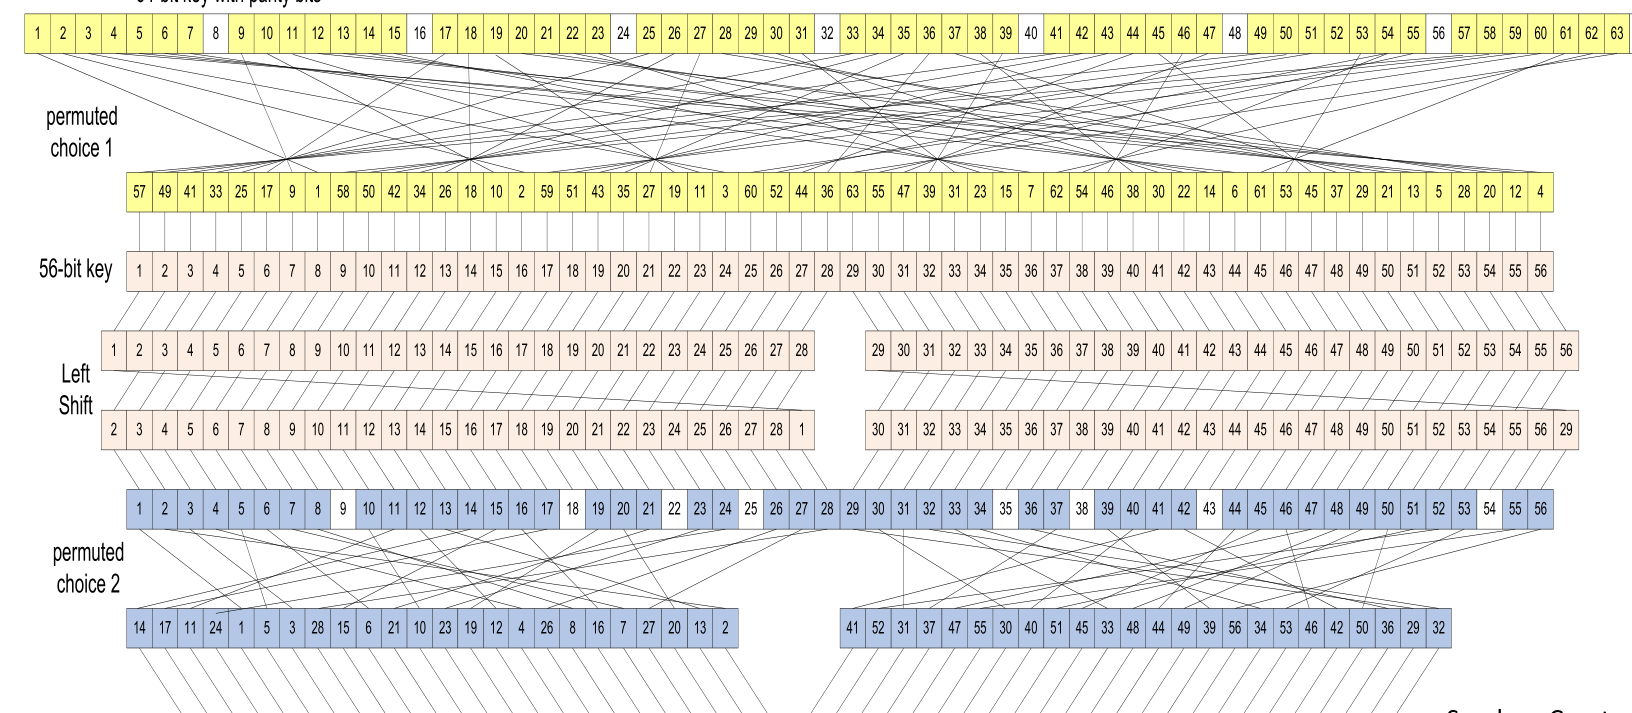
\includegraphics[width=178.50mm,height=196.02mm]{../../images/llm/page_016_img_01.png}%
\end{textblock*}

\end{document}
